\documentclass[dvipsnames]{beamer}
\beamertemplatenavigationsymbolsempty
\usecolortheme{beaver}
\setbeamertemplate{blocks}[rounded=true, shadow=true]
\setbeamertemplate{footline}[page number]
%
\usepackage[utf8]{inputenc}
\usepackage[english,russian]{babel}
\usepackage{amssymb,amsfonts,amsmath,mathtext}
\usepackage{subfig}
\usepackage[all]{xy} % xy package for diagrams
\usepackage{array}
\usepackage{multicol}% many columns in slide
\usepackage{hyperref}% urls
\usepackage{hhline}%tables
\usepackage[dvipsnames]{xcolor}

\graphicspath{ {../figures/} }

%--------------------------------------------------------------------------------------
\title[\hbox to 56mm{Theme}]{Anti-Distillation: Knowledge Transfer from a Simple Model to the Complex One}
\author[K.~Petrushina]{Kseniia Petrushina}
\institute{Moscow~Institute~of~Physics~and~Technology}
\date{\footnotesize
\par\smallskip\emph{Expert:} Vadim~Strijov
\par\smallskip\emph{Consultant:} Andrey Grabovoy
\par\bigskip\small 2022}
%--------------------------------------------------------------------------------------

\begin{document}

%--------------------------------------------------------------------------------------
\begin{frame}
\thispagestyle{empty}
\maketitle
\end{frame}
%--------------------------------------------------------------------------------------

\begin{frame}{Research goal}

    \textbf{Goal}: Adapting the model to more complex data.
    
    \bigskip
    
    Compare uniform initialization with one based on a previously trained model by differences in convergence rate, prediction variance, achieved quality, and stability of the model.

\end{frame}

%--------------------------------------------------------------------------------------

\begin{frame}{Literature}
    \begin{itemize}
        \item Xavier Glorot and Yoshua Bengio. Understanding the difficulty of training deep feed- forward neural networks, 2010.
        \item Geoffrey Hinton, Oriol Vinyals, and Jeff Dean. Distilling the knowledge in a neural network, 2015.
        \item David Lopez-Paz, Léon Bottou, Bernhard Schölkopf, and Vladimir Vapnik. Unifying distillation and privileged information, 2016.
    \end{itemize}
\end{frame}

%--------------------------------------------------------------------------------------

\begin{frame}{Problem statement}
    \newtheorem{hypothesis}{Hypothesis}
    \begin{hypothesis}
    Student models initialized by the result of applying the function $\varphi$ to the weights of the pre-trained teacher model are more persistent and achieve higher accuracy than models with default weights.
    \end{hypothesis}
    
    \bigskip
    
    $D_2 = \{(\textbf{x}_i, y_i)\}_{i=1}^{m_1}$ is \textit{more complex} than $D_1 = \{(\textbf{x}_i, y_i)\}_{i=1}^{m_2}$
    
    \bigskip
    
    Optimal parameters $\hat{\textbf{u}}$ of the teacher model $g$ on $D_1$ dataset are obtained from 
    $$\hat{\mathbf{u}} =  \underset{\mathbf{u}}{\arg\min}~\mathcal{L}_g(\mathbf{u}, D_1),$$
    
    $\mathcal{L}_g(\mathbf{u}, D_1)$ - cross-entropy loss on $D_1$.

\end{frame}

%--------------------------------------------------------------------------------------

\begin{frame}{Problem statement}

    Initialize the student model $f$ weights as $w_1 = \varphi(\hat{\textbf{u}})$.
    
    \bigskip
    
    \textbf{Quality criterions}:
    \begin{itemize}
        \item The value of the loss function on corrupted data.
    
        \item Accuracy of predictions on $D_2$.
    \end{itemize}

\end{frame}

%--------------------------------------------------------------------------------------

\begin{frame}{Problem solution}
    
    Function for weights initialization:
    
    $$\varphi(\mathbf{u}) = \underset{\mathbf{w}}{\arg\min}~\mathcal{L}(\mathbf{w}),$$
 \[\mathcal{L}(\textbf{w}) = \lambda_1 \mathcal{L}_f(\mathbf{w}, D_1^*) + \lambda_2 \mathcal{L}_2 (\mathbf{w}, \mathbf{u}) + \lambda_3 \mathcal{L}_3^\delta (\mathbf{w}, D_1^*) + \lambda_4 \mathcal{L}_4 \bigl(\displaystyle \frac{\partial^2 \mathcal{L}_f}{\partial \mathbf{w}^2}\bigr).\]

    \begin{itemize}
        \item $\mathcal{L}_2 (\mathbf{w}, \mathbf{u}) = \|\textbf{u} - \textbf{w}[\textbf{u}]\|^2_2$
        \item $\mathcal{L}_3^\delta (\mathbf{w}, D_1^*) = \displaystyle \sum \limits_{(\textbf{x}, y) \in D_1^*} \displaystyle \mathbb{E}_{\textbf{x}' \in U_\delta(\textbf{x})} \mathcal{L}_f(\mathbf{w}, \textbf{x}', y)$
        \item $\mathcal{L}_4 \bigl(\displaystyle \frac{\partial^2 \mathcal{L}_f}{\partial \mathbf{w}^2}\bigr) = \|\bigl(\displaystyle \frac{\partial^2 \mathcal{L}_f}{\partial \mathbf{w}^2}\bigr)\|^2_2$
    \end{itemize}

\end{frame}

%--------------------------------------------------------------------------------------

\begin{frame}{Computational experiment}

    \textbf{Goal}: Compare the performance of models depending
on the initialization of parameter
    
    \begin{columns}[c]
    \column{0.75\textwidth}
    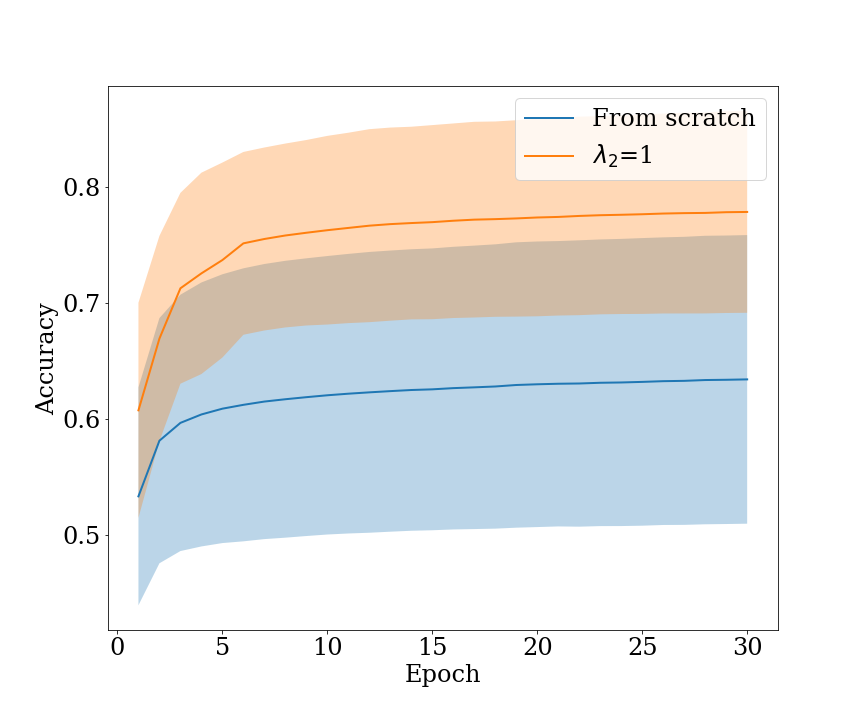
\includegraphics[width=\textwidth]{l2_acc.png}
    \column{0.5\textwidth}
    $\mathbf{w}_1 = \varphi(\mathbf{u}^*)$ \\
    \bigskip
    $\mathbf{w}_1 = (\mathbf{u}^*, \mathbf{w}_1'), $ \\
    \bigskip
    $\mathbf{w}_1' \sim {\color{orange} U[-\frac{1}{\sqrt{n}}, \frac{1}{\sqrt{n}}]}$
    
    \end{columns}

\end{frame}

%--------------------------------------------------------------------------------------

\begin{frame}{Conclusion}

    A new method for parameters initialization of fully-connected neural newtorks, which helps to achieve higher accuracy on \textit{more complex} dataset.

    \bigskip

    \textbf{Next}: CNN and RNN, different default parameters initialization.

\end{frame}

%--------------------------------------------------------------------------------------

\end{document} 